%
\hsection{\crowsFoot{Q}{OM}{R}{MM}}%
\label{sec:rm:qr}%
%
\begin{figure}%
\centering%
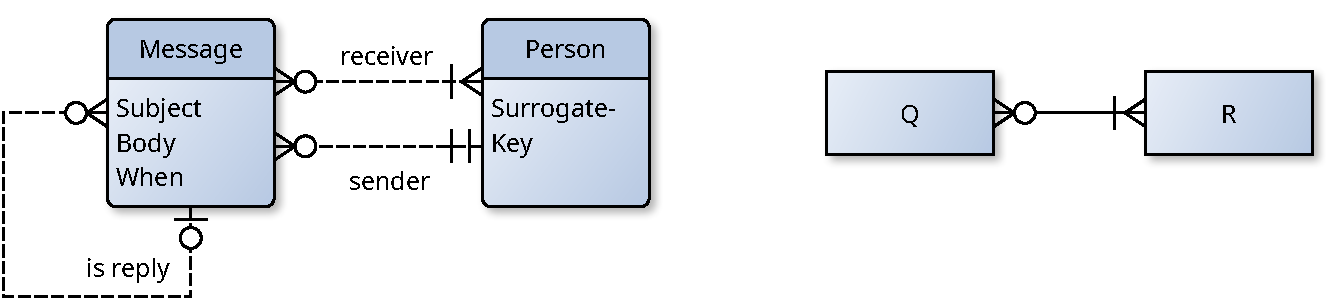
\includegraphics[width=0.9\linewidth]{\currentDir/QR}%
\caption{We encountered the \crowsFoot{Q}{OM}{R}{MM} relationship pattern in \cref{fig:erdMessage1}.}%
\label{fig:rm:qr}%
\end{figure}%
%
\gitLoadAndExecSQL{QR_tables}{}{conceptualToRelational}{QR_tables.sql}{relationships}{}{}%
\listingSQLandOutput{QR_tables}{QR_tables.sql}{%
The realization of a \crowsFoot{Q}{OM}{R}{MM} conceptual relationship.%
}{}%
%
\gitLoadAndExecSQL{QR_insert_and_select}{}{conceptualToRelational}{QR_insert_and_select.sql}{relationships}{}{}%
\listingSQLandOutput{QR_insert_and_select}{QR_insert_and_select.sql}{%
Inserting into and selecting data from the realization of an \crowsFoot{Q}{OM}{R}{MM} conceptual relationship given in \cref{lst:QR_tables}.%
}{}%
%
\gitExec{cdtrmTableQ}{\databasesCodeRepo}{conceptualToRelational}{../_scripts_/db_table_to_latex_table.sh relationships q qid;fkrid;x}%
\gitExec{cdtrmTableR}{\databasesCodeRepo}{conceptualToRelational}{../_scripts_/db_table_to_latex_table.sh relationships r rid;y}%
\gitExec{cdtrmTableRQR}{\databasesCodeRepo}{conceptualToRelational}{../_scripts_/db_table_to_latex_table.sh relationships relate_q_and_r fkqid;fkrid}%
%
\begin{figure}%
\centering%
\floatSep%
\input{\gitFile{cdtrmTableQ}}%
\floatSep%
\input{\gitFile{cdtrmTableR}}%
\floatSep%
\input{\gitFile{cdtrmTableRQR}}%
\floatSep%
\caption{The contents of the the three tables in the implementation of the \crowsFoot{Q}{OM}{R}{MM} conceptual relationship after executing \cref{lst:QR_insert_and_select}.}%
\label{fig:rm:qr:tables}%
\end{figure}%
%
\gitLoadAndExecSQL{QR_insert_error_1}{}{conceptualToRelational}{QR_insert_error_1.sql}{relationships}{}{}%
\listingSQLandOutput{QR_insert_error_1}{QR_insert_error_1.sql}{%
Trying to create a row into table~\sqlil{q} without providing a foreign key to a row in~\sqlil{r} fails.%
}{}%
%
\gitLoadAndExecSQL{QR_insert_error_2}{}{conceptualToRelational}{QR_insert_error_2.sql}{relationships}{}{}%
\listingSQLandOutput{QR_insert_error_2}{QR_insert_error_2.sql}{%
Trying to create a row into table~\sqlil{q} with creating a corresponding row in table~\sqlil{relate_q_and_r} also fails.%
}{}%
%
\gitLoadAndExecSQL{QR_insert_error_3}{}{conceptualToRelational}{QR_insert_error_3.sql}{relationships}{}{}%
\listingSQLandOutput{QR_insert_error_3}{QR_insert_error_3.sql}{%
Even if we can choose the primary key for the new row in table~\sqlil{q}, we cannot create the associated row in table~\sqlil{relate_q_and_r} first.%
}{}%
%
We have the two entity types~Q and~R.
Each entity of type~Q may be connected to zero, one, or multiple entities of type~R.
Each entity of type~R must be connected to at least one entity of type~P, but can be connected to many.

We came across this situation when modeling the messaging subsystem of our teaching management platform back in \cref{fig:erdMessage1}.
A message must have at least one receiver, but it could also be sent to multiple people at once.
Each person may receive zero, one, or many messages.
This situation is sketched in \cref{fig:rm:qr}.

Let us again begin by establishing the basic tables that we need and then sort out how we can enforce referential integrity with proper constraints.
We need a table~\sqlil{q} for the entities of type~Q.
The primary key of this table be~\sqlil{qid} and there also will be the example attribute~\sqlil{x}.
We also need a table~\sqlil{r} for the entities of type~R, which gets the primary key~\sqlil{rid} and the example attribute~\sqlil{y}.
Since both ends of the relationship allow for a row to be connected to multiple rows in the other table, we definitely will need three tables.

We create another table~\sqlil{relate_q_and_r} to manage the relationships in \cref{lst:QR_tables}.
This table has two columns,~\sqlil{fkqid} and~\sqlil{fkrid}, which are foreign keys pointing to the primary keys~\sqlil{qid} and~\sqlil{rid} of tables~\sqlil{q} and~\sqlil{r}, respectively.
This is ensured with corresponding \sqlil{REFERENCES} constraints.
Both columns are marked as~\sqlil{NOT NULL}.
Like in \cref{sec:rm:op}, each pair~\sqlil{(fkqid, fkrid)} can appear only once in the table, because two specific rows in tables~\sqlil{q} and~\sqlil{r} can, of course, be related only once to each other.
This is implemented via the constraint~\sqlil{PRIMARY KEY (fkqid, fkrid)}.

Compared to \cref{sec:rm:op}, the problem that we need to solve is that we must force that each row in table~\sqlil{q} is related to (at least) one row in table~\sqlil{r}.
Back in \dref{sec:rm:gh}, we faced a similar problem, i.e., \inQuotes{How can we make sure that each entity of type~G is connected to at least one entity of type~H?}
The main problem there was not to make a new row in table~\sqlil{g} reference some row in table~\sqlil{h}, but that we then must make that row in table~\sqlil{h} reference back the same row in table~\sqlil{g}.
We solved this by creating a constraint that enforced that the primary key of that row in table~\sqlil{h} together with the foreign key to the table~\sqlil{q} would need to be the same as the foreign key of the row in table~\sqlil{q} and its primary key.

Now our relationships are managed in the table~\sqlil{relate_q_and_r}.
What we need to do is to make sure that, if we insert a row into table~\sqlil{q}, we must also -- at the same time -- insert a row into table~\sqlil{relate_q_and_r} that will link this row to a row in table~\sqlil{r}.
We again store a \inQuotes{primary R} foreign key to a row in~\sqlil{r} as column~\sqlil{fkrid} in table~\sqlil{q}.
Then we add the constraint~\sqlil{q_qid_fkrid_fk} to table~\sqlil{q} which enforces~\sqlil{FOREIGN KEY (qid, fkrid) REFERENCES relate_q_and_r (fkqid, fkrid)}.

In \cref{lst:QR_insert_and_select}, we now insert data into the two tables.
For the entities of type~R, the connection to entities of type~Q is optional.
Therefore, we can populate the table~\sqlil{r} first.

If we want to insert a row into table~\sqlil{q}, however, we must at the same time also insert a row into table~\sqlil{relate_q_and_r}.
When we do this, the new row in table~\sqlil{relate_q_and_r} must use the primary key of the new row in table~\sqlil{q} as foreign key.
This means that we will again use a \pgls{CTE}, which we will call~\sqlil{q_new}.
We define it as \sqlil{INSERT INTO q (x, fkrid) VALUES ('123', 1) RETURNING qid, fkrid}.
Here, we want to insert a row into table~\sqlil{q} whose \sqlil{x}~attribute has value~\sqlil{'123'} and that is related to the entry with primary key~\sqlil{1} in table~\sqlil{r}.
Once this insert is executed, it will return the primary key of the new row~(as \sqlil{qid}) and the foreign key to the row in table~\sqlil{r}, which is named~\sqlil{fkrid} and obviously has value~\sqlil{1}.%
%
\begin{sloppypar}%
This \pgls{CTE} is then used to insert a new row into table~\sqlil{relate_q_and_r}.
We write \sqlil{INSERT INTO relate_q_and_r (fkqid, fkrid) SELECT qid, fkrid FROM q_new;}.
This is pretty straightforward:
The new row in table~\sqlil{relate_o_and_p} gets the primary key to the new row in table~\sqlil{q} as well as the primary key of the row in table~\sqlil{r} that it references.
Both insertions are executed as one single command and the referential integrity constraints are checked at its end.%
\end{sloppypar}%
%
We insert a few rows into tables~\sqlil{q} and~\sqlil{relate_q_and_r} using this method.
Once this is done, we can easily add more connections as rows in table~\sqlil{relate_q_and_r}.
The contents of all three tables after we inserted the data are displayed in \cref{fig:rm:qr:tables}.
Finally, we can merge the data again using the same two \sqlil{INNER JOIN} expressions we used several times before.

It is clear that we cannot insert any row into table~\sqlil{q} that does not provide a foreign key to a row in table~\sqlil{r}, as shown in \cref{lst:QR_insert_error_1}.
Neither can we insert a row that does provide such a foreign key, but for which now row in table~\sqlil{relate_q_and_r} exists, as shown in \cref{lst:QR_insert_error_2}.
Finally, \cref{lst:QR_insert_error_3} shows that we can also not first insert a row into table~\sqlil{relate_q_and_r} and then create the corresponding row in table~\sqlil{q}, even if we know the right primary key for that second new row.
In other words, our constraints properly protect the referential integrity of the relationship pattern.%
%
\FloatBarrier%
\endhsection%
%
